\documentclass[../masterarbeit.tex]{subfiles}
\begin{document}
	



\subsection{Performance Evaluation}
The Evaluation of machine learning models is core part of building an effective and robust model. It is not only a technique to get feedback, at the end of a machine learning training process, which shows how good the quality of the models results are. The performance evaluation is also part of the optimization process while training a machine learning model. This can be an iterative process, in which a model is trained, after that feedback of quality is obtained through metrics, then the models hyper-parameters or features are improved (depending on the actual phase of process of creating a machine learning model) and this is repeated until a solid model has been found. \autocite[]{analyticsvidhya_evaluation:2022} \\
The metrics used to evaluate supervised machine learning models are also divided into evaluation of classification and regression models \textcite[]{jeremyjordan_evaluation:2022}. Causing the fact that the prediction problem of this study is a classification problem, only evaluation metrics which are used to evaluated classifier models are mentioned in this topic. \\
The outcome of a binary machine learning classifier prediction has one of the four following types \textcite[]{jeremyjordan_evaluation:2022}:
\begin{itemize}
	\item True positive (TP): The model predicts that an observation belongs to a class and it actually belongs to that class.
	\item False positive (FP): The model predicts that an observation belongs to a class and it actually does not belong to that class.
	\item True negative (TN): The model predicts that an observation not belongs to a class and it does not belog to that class.
	\item False negative (FN): The model predicts that an observation not belongs to a class and it does belog to that class.
\end{itemize} 
This four values can be plotted on a confusion matrix. An example for that matrix is shown in Figure 8. The matrix is generated by making predictions on the test data and assigning the results of the individual samples to the four types. Also different classification model evaluation metrics, like the three main scores accuracy, precision and recall score are calculated with these values. \autocite[]{jeremyjordan_evaluation:2022}


\begin{figure}[h]
    \centering
    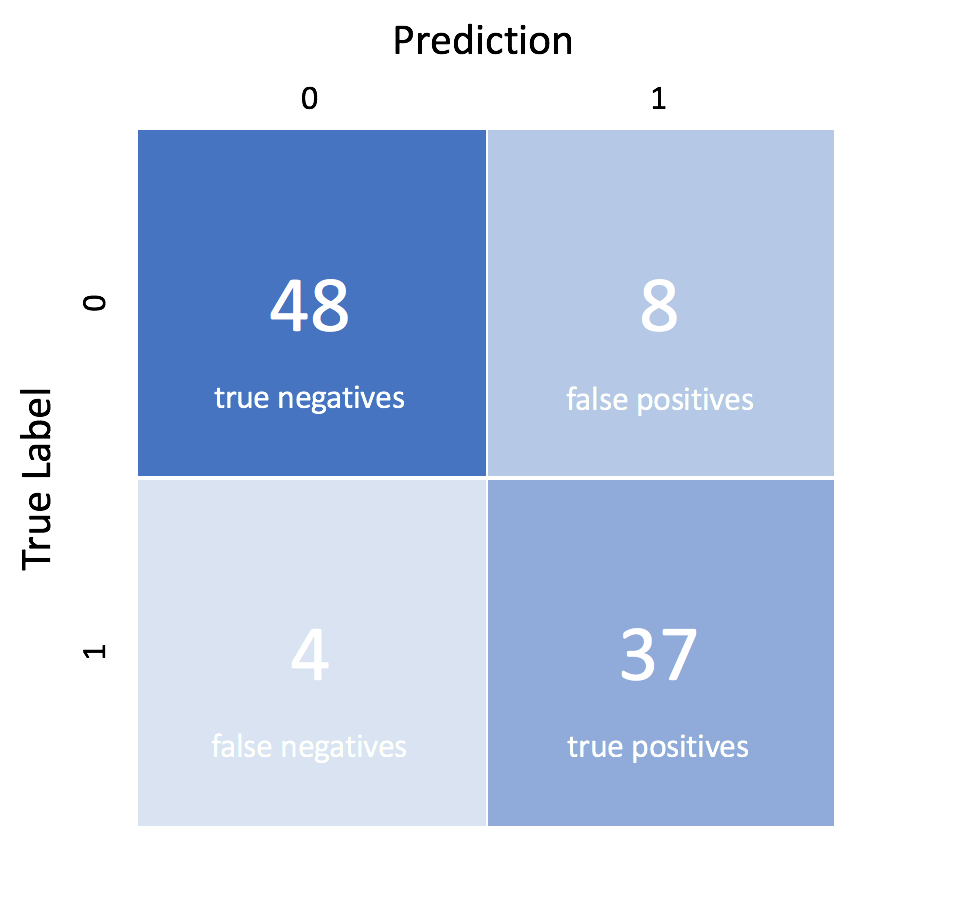
\includegraphics[scale=0.6]{confusion_matrix_example.png}
    \source{\autocite[]{jeremyjordan_evaluation:2022}}
    \caption{A confusion matrix which shows the four types of a classifier outcomes.}
\end{figure} \\









\subsubsection{Accuracy}
The Accuracy score is one of the most common evaluation metrics, when it comes to the evaluation of binary classifiers \textcite[]{Kartik_evaluation:2022}. Also a lot of the related works use this score to evaluate and compare their machine learning models. Jeremy Jordans defines accuracy as follows:
\begin{quote}
	"Accuracy is defined as the percentage of correct predictions for the test data." \autocite{jeremyjordan_evaluation:2022}
\end{quote}
The definition can also be represented like this: 
\\
\(Accuracy = \frac{Number of correct predictions}{Number of total predictions} \) \hfill \textcite[]{Google_Acurracy:2022} \\~\\
For binary classifiers accuracy is can be calculated as follows: \\
\(Accuracy = \frac{TP + TN}{TP + FP + TN + FN} \) \hfill \textcite[]{Kartik_evaluation:2022} \\~\\
As the definitions describe, the score represents the percentage of the correctness of all predictions. This implies that in the case of an unbalanced class size, the accuracy of a class can be disregarded \textcite[]{Kartik_evaluation:2022}. As an example in the context of avalanche prediction: There are 90 samples that do not contain an avalanche event and only 10 which represent an avalanche event. In the case that the algorithm predicts no avalanche event for all samples, it has an accuracy of 90\%. \\
This does not mean that the accuracy score is not useful, the metrics gives a validation of the overall prediction performance of the model. It only signifies that it should not be the only score used for the evaluation, especially in cases of unbalanced class sizes. \autocite[]{Google_Acurracy:2022} \\~\\
For datasets, which classes are not balanced, the pyhton library Sklearn.metrics includes a more balanced version of the accuracy score called balanced accuracy score. For a binary classification, this score weights the class which is less represented in the datasets more than the other one. This can indicate if the machine learning algorithm is biased by the more represented class of the dataset. \autocites{Scikit-model-evaluation:2022}
This balanced accuracy score is calculated for binary classification problems as follows: \\~\\
\(Balanced Accuracy = \frac{1}{2}(\frac{TP}{TP + FN} + \frac{TN}{TN + FP}) \) \hfill \textcite[]{Scikit-model-evaluation:2022} \\~\\
In the case of a biased machine learning model, the normal accuracy might be higher value than the balanced one. The range of the resulting score is between 0 and 1. While the score is 0.0 if all predictions are wrong, 0.5 if the predictions are chance and 1.0 if the predictions are all true. The score can be performed on binary and multiclass classification problems. The score is defined as the average of the recall score, explained in section 3.4.3, calculated for ever class of the dataset.\autocites{Scikit-model-evaluation:2022}
For the later interpretation of the accuracy score, a basic assessment of which values can be recognized as good should be given. Even though it depends very much on what one wants to predict with machine learning, what a good prediction quality means, Kirsten Barkved \textcite[]{obviously.ai:2022} describes in her article all models whose accuracy score lies between 70\% and 90\% as good and above all realistic.






\subsubsection{Precision}
The Precision score is the percentage of how many positive predicted observations actually are positive \textcite[]{Kartik_evaluation:2022}. The score is calculated by dividing the number of positive predicted samples that are actually positive by the total number of positive predicted samples \textcite[]{Kartik_evaluation:2022}. So it calculates the false rated actual negative values into the score. If all positive rated values are actual positive, the score is 1.0 and if all are negative, the score is 0.0. The score is 0.5 if the prediction is chance.\\
It is calculated as follows:
\\~\\
\(Precision = \frac{TP}{TP + FP} \) \hfill \textcite[]{Kartik_evaluation:2022} \\~\\
The score can be a balancing validation metric for the accuracy score, since it covers exactly the cases in which the accuracy score has the problem described above. So to extend the example mentioned in section 3.3.1, in which the Number of Avalanches is 10 and ne number of non avalanches is 90. The model only predicts all non-avalanches correctly so the accuracy is 90\% but the precision score is 0\%. So in this case the accuracy shows that the model has a high prediction quality, but the precision score clarifies that none of the avalanches was predicted.\\
The fact the use of the Precision Score without the evaluation with another metric, has a similar problem \autocite[]{Google_Precision_Recall:2022}. In case of the example if only one positive samples is correctly predicted as avalanche, the precision score is 100\% but nine of ten avalanche samples are rated false. So the same balancing characteristic applies the other way around from accuracy score to precision score. Figure 9 shows a set of datapoints. The precision score evaluates the right side of the classification threshold line. Since the precision score only targets the samples predicted as positive. In the case shown in figure 9, seven out of 8 datapoints are predicted right, which results in a precision score of 0.875.



\begin{figure}[h]
    \centering
    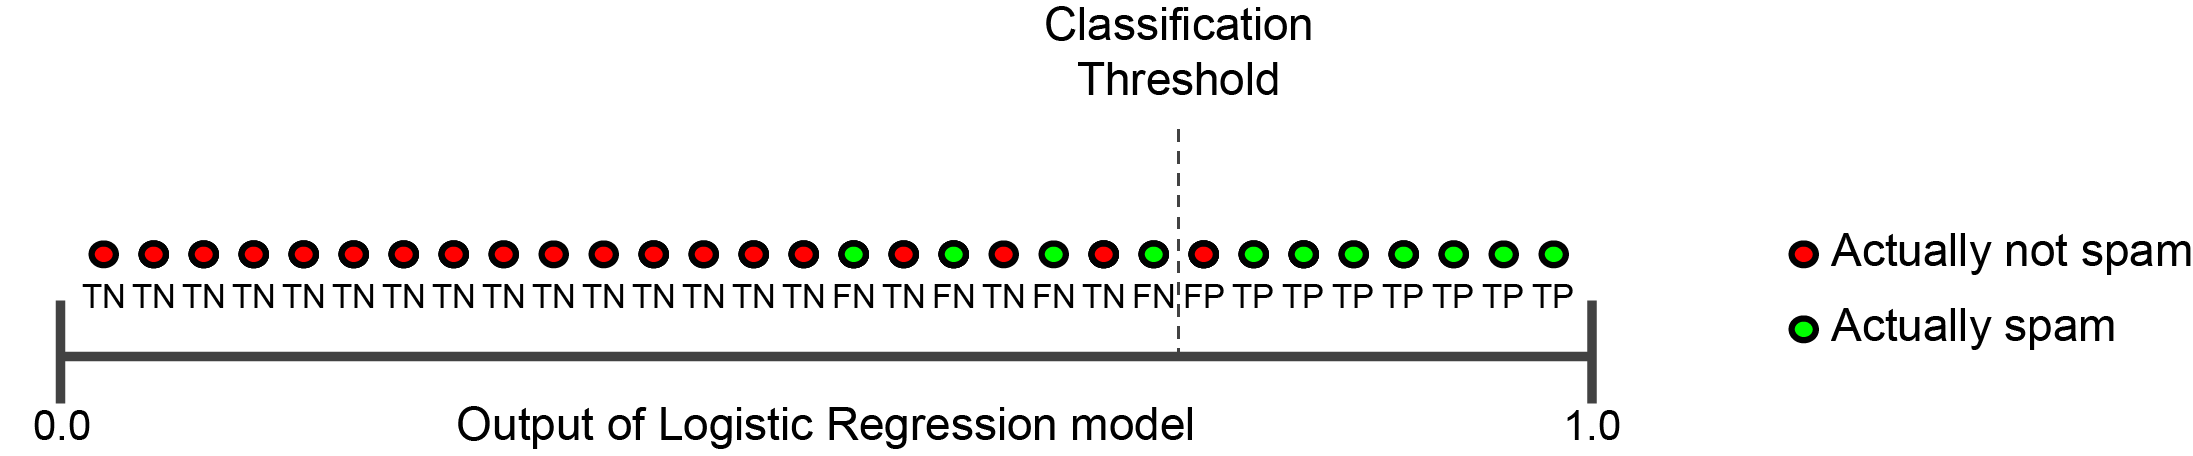
\includegraphics[scale=0.9]{PrecisionVsRecallRaiseThreshold.png}
    \source{\autocite[]{Google_Precision_Recall:2022}}
    \caption{A set of datapoints split by the classifier and marked as one of the four classifier output types.}
\end{figure} 


\subsubsection{Recall}
The Recall is another evaluation score, calculated out of the four values represented in the confusion matrix. It is defined as the percentage of actual positive datapoints predicted as positive \textcite[]{Google_Precision_Recall:2022}. In figure 9 the recall is represented as all green marked datapoints on the right sight (the TP predicted samples) of the classification threshold line divided by the all green marked samples (the TP plus FN predicted samples). \\
The recall score, which is also known as True-Positve-Rate, is calculated by dividing the True-Positive output values through the through all actual positive values. If no positive samples are predicted correctly, the recall score is zero and if all actual positive samples are predicted correctly, the recall score is 1.0. Similar to the accuracy and precision, if the recall score is 0.5 its chance.
The recall evaluation metric is calculated as follows:
\\~\\
\(Recall = \frac{TP}{TP + FN} \) \hfill \textcite[]{Kartik_evaluation:2022} \\~\\


\subsubsection{ROC-Curve and AUC}
The ROC curve (Receiver operating characteristic) is a graph representing the True Positive Rate (TPR) compared to the False Positive Rate (FPR) for different classification thresholds of a model \textcite[]{Google_ROC_AUC:2022}. In figure 10 an example ROC curve is shown. Each dot on the curve represents the TP vs. the FP rate at a specific decision threshold.\\
As with the calculation of the recall score, the True-Positive-Rate compares the number of correctly positive predicted samples with the total number of positive samples. The False-Positive-Rate represents the number of falsely positive predicted samples compared to the total number of negative values. 
The calculations of the two parameters TPR and FPR are defined in mathematical notation as follows:
\\~\\
\(TPR = \frac{TP}{TP + FN} \) \hfill \textcite[]{Google_ROC_AUC:2022} \\~\\
\(FPR = \frac{FP}{FP + TN} \) \hfill \textcite[]{Google_ROC_AUC:2022} 
\\~\\
As the two parameters TPR and FPR show, all four output types are represented in the ROC curve.
If the threshold is lower, the model classifies more samples as positive. The consequence of this is that both the TPR and the FPR increase. The same happens in reverse with a higher threshold. The perfect ROC-curve does go straight up to 1 and then straight to the right. So in this case the model would predict the samples perfectly. \autocite[]{Google_ROC_AUC:2022} \autocite[]{Kartik_evaluation:2022} \\
For machine learning classifiers, which have a class as output and do not use a threshold, the ROC curve will be represented as a single point in the plot \textcite[]{analyticsvidhya_evaluation:2022}. \\ 

\begin{figure}[h]
    \centering
    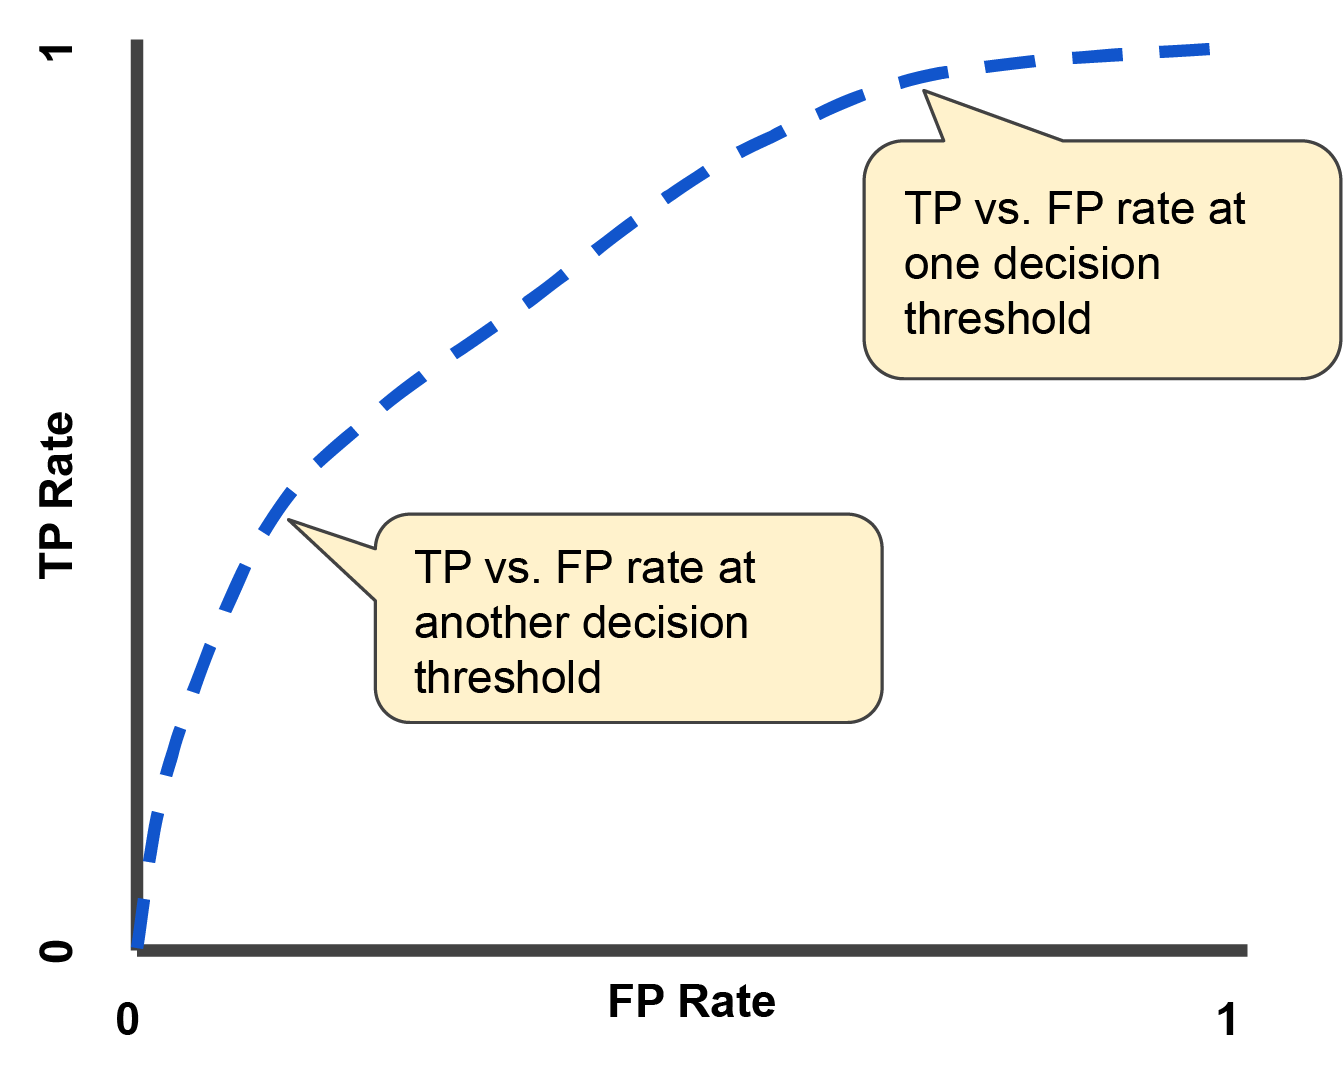
\includegraphics[scale=0.6]{ROCCurve.png}
    \source{\autocite[]{Google_ROC_AUC:2022}}
    \caption{The ROC curve plots the TPR vs. the FPR on all different thresholds.}
\end{figure}
An interactive approach, in which a classifier model is evaluated many times with different thresholds, would be associated with high computational costs. However, there is also a more efficient approach called AUC, which can also determine this information. \autocite[]{Google_ROC_AUC:2022} \\~\\


The AUC (Area under the Curve) statistic represents the integral calculus of the ROC curve from (0,0) to (1,1). Figure 11 shows an example for the AUC statistic. The grey marked area in that figure represents the AUC value of this ROC curve. It gives an aggregate measure of the models prediction quality about the whole range of possible classification thresholds. So with the AUC statistic, the ROC curve is represented by a single number. The value of AUC can be in the range between 0 and 1. If the Value is 0.0, the predictions are 100\% false. If the value is 1.0, all predictions are correct. If the value is below 0.5 the predictions of the model are below chance, because chance is represented by the value of 0.5 \autocites[]{Google_ROC_AUC:2022, analyticsvidhya_evaluation:2022} The value The higher the numerical values of the AUC statistic the better is the models performance \textcite[]{analyticsvidhya_evaluation:2022}. This number is definitely meaningful, however, the entire ROC curve should always be considered as there are models that perform better in certain areas and other models in other regions \textcite[]{analyticsvidhya_evaluation:2022}. 
An AUC value between 0.7 and 0.8 is considered as acceptable, while an AUC value between 0.8 and 0.9 is rated as excellent and above 0.9 it is classified as outstanding \textcite[]{MANDREKAR20101315}\\




\begin{figure}[h]
    \centering
    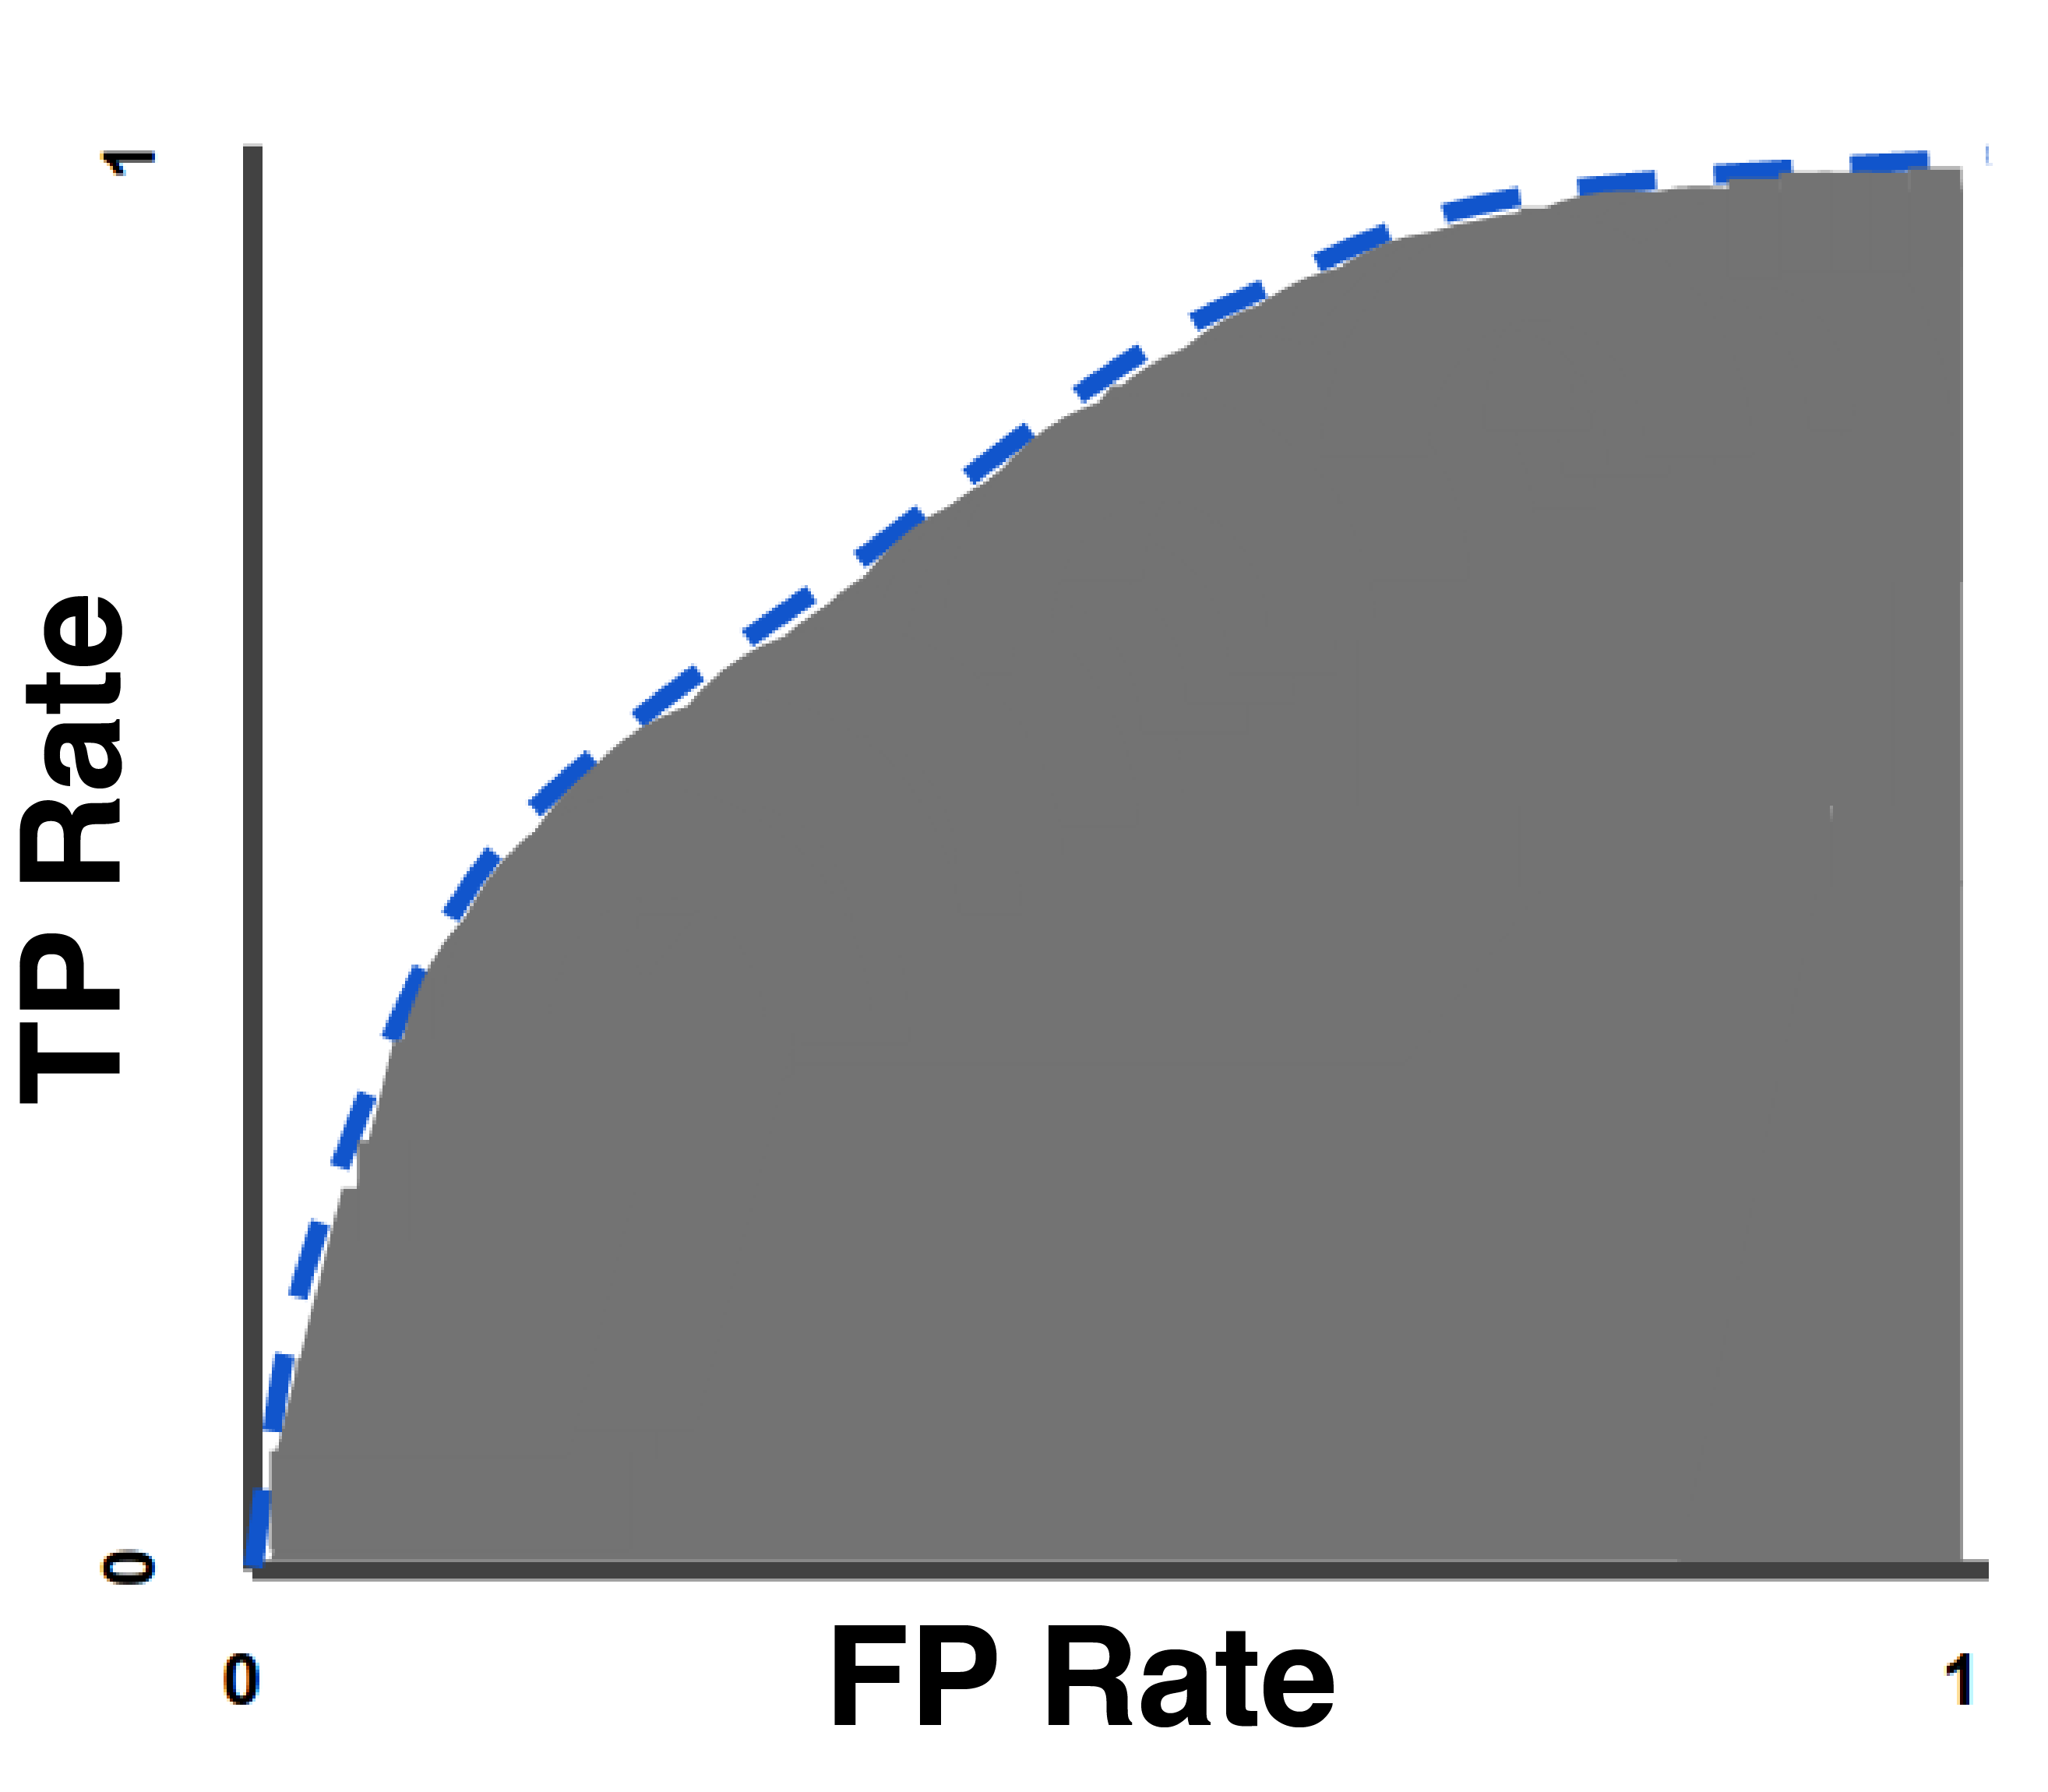
\includegraphics[scale=0.3]{AUC.png}
    \source{\autocite[]{Google_ROC_AUC:2022}}
    \caption{The AUC statistic represents the grey marked area under the ROC curve.}
\end{figure} \\

In Context of this work, the implementation of the ROC-curve as well as the AUC value included in the same python library (Sklearn.metrics) as the other metrics mentioned before are used. This implementation of the ROC-curve is restricted to binary classification tasks. \autocite[]{Scikit-learn-roc-curve:2022}



\subsubsection{K-Fold Cross-Validation}

The k-fold cross-validation is a technique to evaluate machine learning classifier models in a balanced way and to avoid the risk of a random training test split variant with a splitting that is not meaningful. This balance is caused by the fact that with this method the model is both trained and validated with every data sample of the set. \autocite[]{Refaeilzadeh2009} \\
In the k-fold cross-validation, the dataset is split into k equally sized subsets. After that the model is trained iteratively with k-1 folds of the dataset and the last fold is used for validation. The one fold which is held-out change every iteration until the model is validated with every sample of the set. The performance of each iteration is tracked by an evaluation metric like accuracy or precision. This process is shown for the example of an 5-fold cross validation in figure 12. In the figure, the test set is the orange and the training set is the yellow marked part of the set. As shown, this test part always shifts by one fifth of the total set. \autocite[]{Refaeilzadeh2009} \\
\begin{figure}[h]
    \centering
    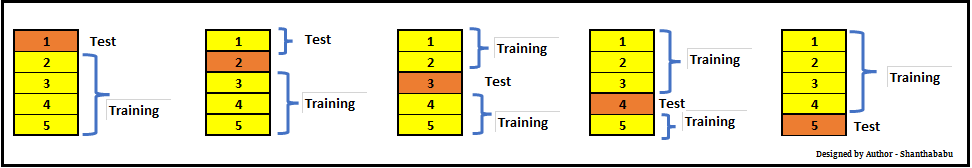
\includegraphics[scale=0.6]{K-fold.png}
	\source{\autocite[]{analyticsvidhya_cross_validation:2022}}    
    \caption{The iteration process of a 5-fold cross-validation.}
\end{figure}
The 10-fold cross validation is a popular variant in terms of machine learning. the decisive advantage compared to, for example, a 70/30 train test split is that you have a large train set of 90\% for each iteration. So the machine learning model does have more samples to learn from. At the same time k-fold cross-validation provides a precise test coverage. \autocite[]{analyticsvidhya_cross_validation:2022}
In the case of this master thesis, the accuracy, precision and recall metric are all used in combination with the cross-validation implementation of the Python library sklearn.model\_selection, in which the metrics can be selected. 


























\end{document}